\section*{Experiment Design}

\subsection*{Hypothesis}

As the current going through the wire increase, the force acting on the wire due to a magnetic field will linearly increase. Hence, the deflection angle of the pendulum apparatus will also increase.

\subsection*{Variables}

\textbf{Independent variable} --- current flowing through the wire of the pendulum, achieved through varying output voltage from the power supply.
Due to the inconsistent resistance of the circuit, caused by changing contact of the wire with the supports as it swings, exact current values cannot be achieved.
The target current values were $0.20\si{\ampere}$, $0.40\si{\ampere}$, $0.60\si{\ampere}$, $0.80\si{\ampere}$, $1.00\si{\ampere}$, $1.20\si{\ampere}$, and $1.40\si{\ampere}$.
These variables were measured with an uncertainty of $\pm0.01$ based off the readings from the power supply.

\textbf{Dependent variable} --- angle of deflection of the pendulum. The angle was measured through by imaging the deflecting pendulum at a flat plane and constant distance, then using a measurement tool from GIMP, an image processing software. The measurement uncertainty was $\pm0.01$.

\textbf{Controlled variables} --- the mass of the wire; $4.9\pm0.1\si{\gram}$ --- length of the copper wire under the magnetic field; $4.61\pm0.05\si{\centi\meter}$ --- pendulum length; $5.56\pm0.05\si{\centi\meter}$ --- distance between magnets; $3.12\pm0.05\si{\centi\meter}$.
The wire is kept perpendicular to the magnetic field lines between the magnets.

\subsection*{Procedure}

\begin{enumerate}
	\item Gather a breadboard, two straightened, conductive, identical paper clips, needle nose pliers, and a spool of exposed copper wire to create the pendulum.
	\begin{enumerate}
		\item Using needle nose pliers, take the end of a straightened paper clip and bend it into a knuckle that will act as a pivot for the pendulum wire.
		Create a knuckle on the other paper clip such that the length of both paper clips are the same.
		Ensure the knuckles overhang so that there is enough clearance between the knuckles and the wire when it is placed.
		Place both paper clips at least $4\si{\centi\meter}$ away from each other on the breadboard; they will act as supports for the wire.
		\item Spool out an appropriate length of copper wire so that there is at least $5\si{\centi\meter}$ of length between the pivot and the lowest point of the wire.
		At least $15\si{\centi\meter}$ of wire should be used, with excess being used to secure the wire to the supports. 
		Using needle nose pliers, bend the ends of the wire into a U shape hook to allow the wire to hang from the supports.
		Bend the remaining wire into a square U shape such that the vertical segments are of equal length and the horizontal segment is roughly equal to the distance between the supports.
		\item Fit the wire into the supports and check if it can swing freely.
		If the wire does not swing freely, either minutely unbend the knuckles on the supports or widen the U shape hooks at the end of the wire.
	\end{enumerate}
	\begin{figure}[H]
		\centering
		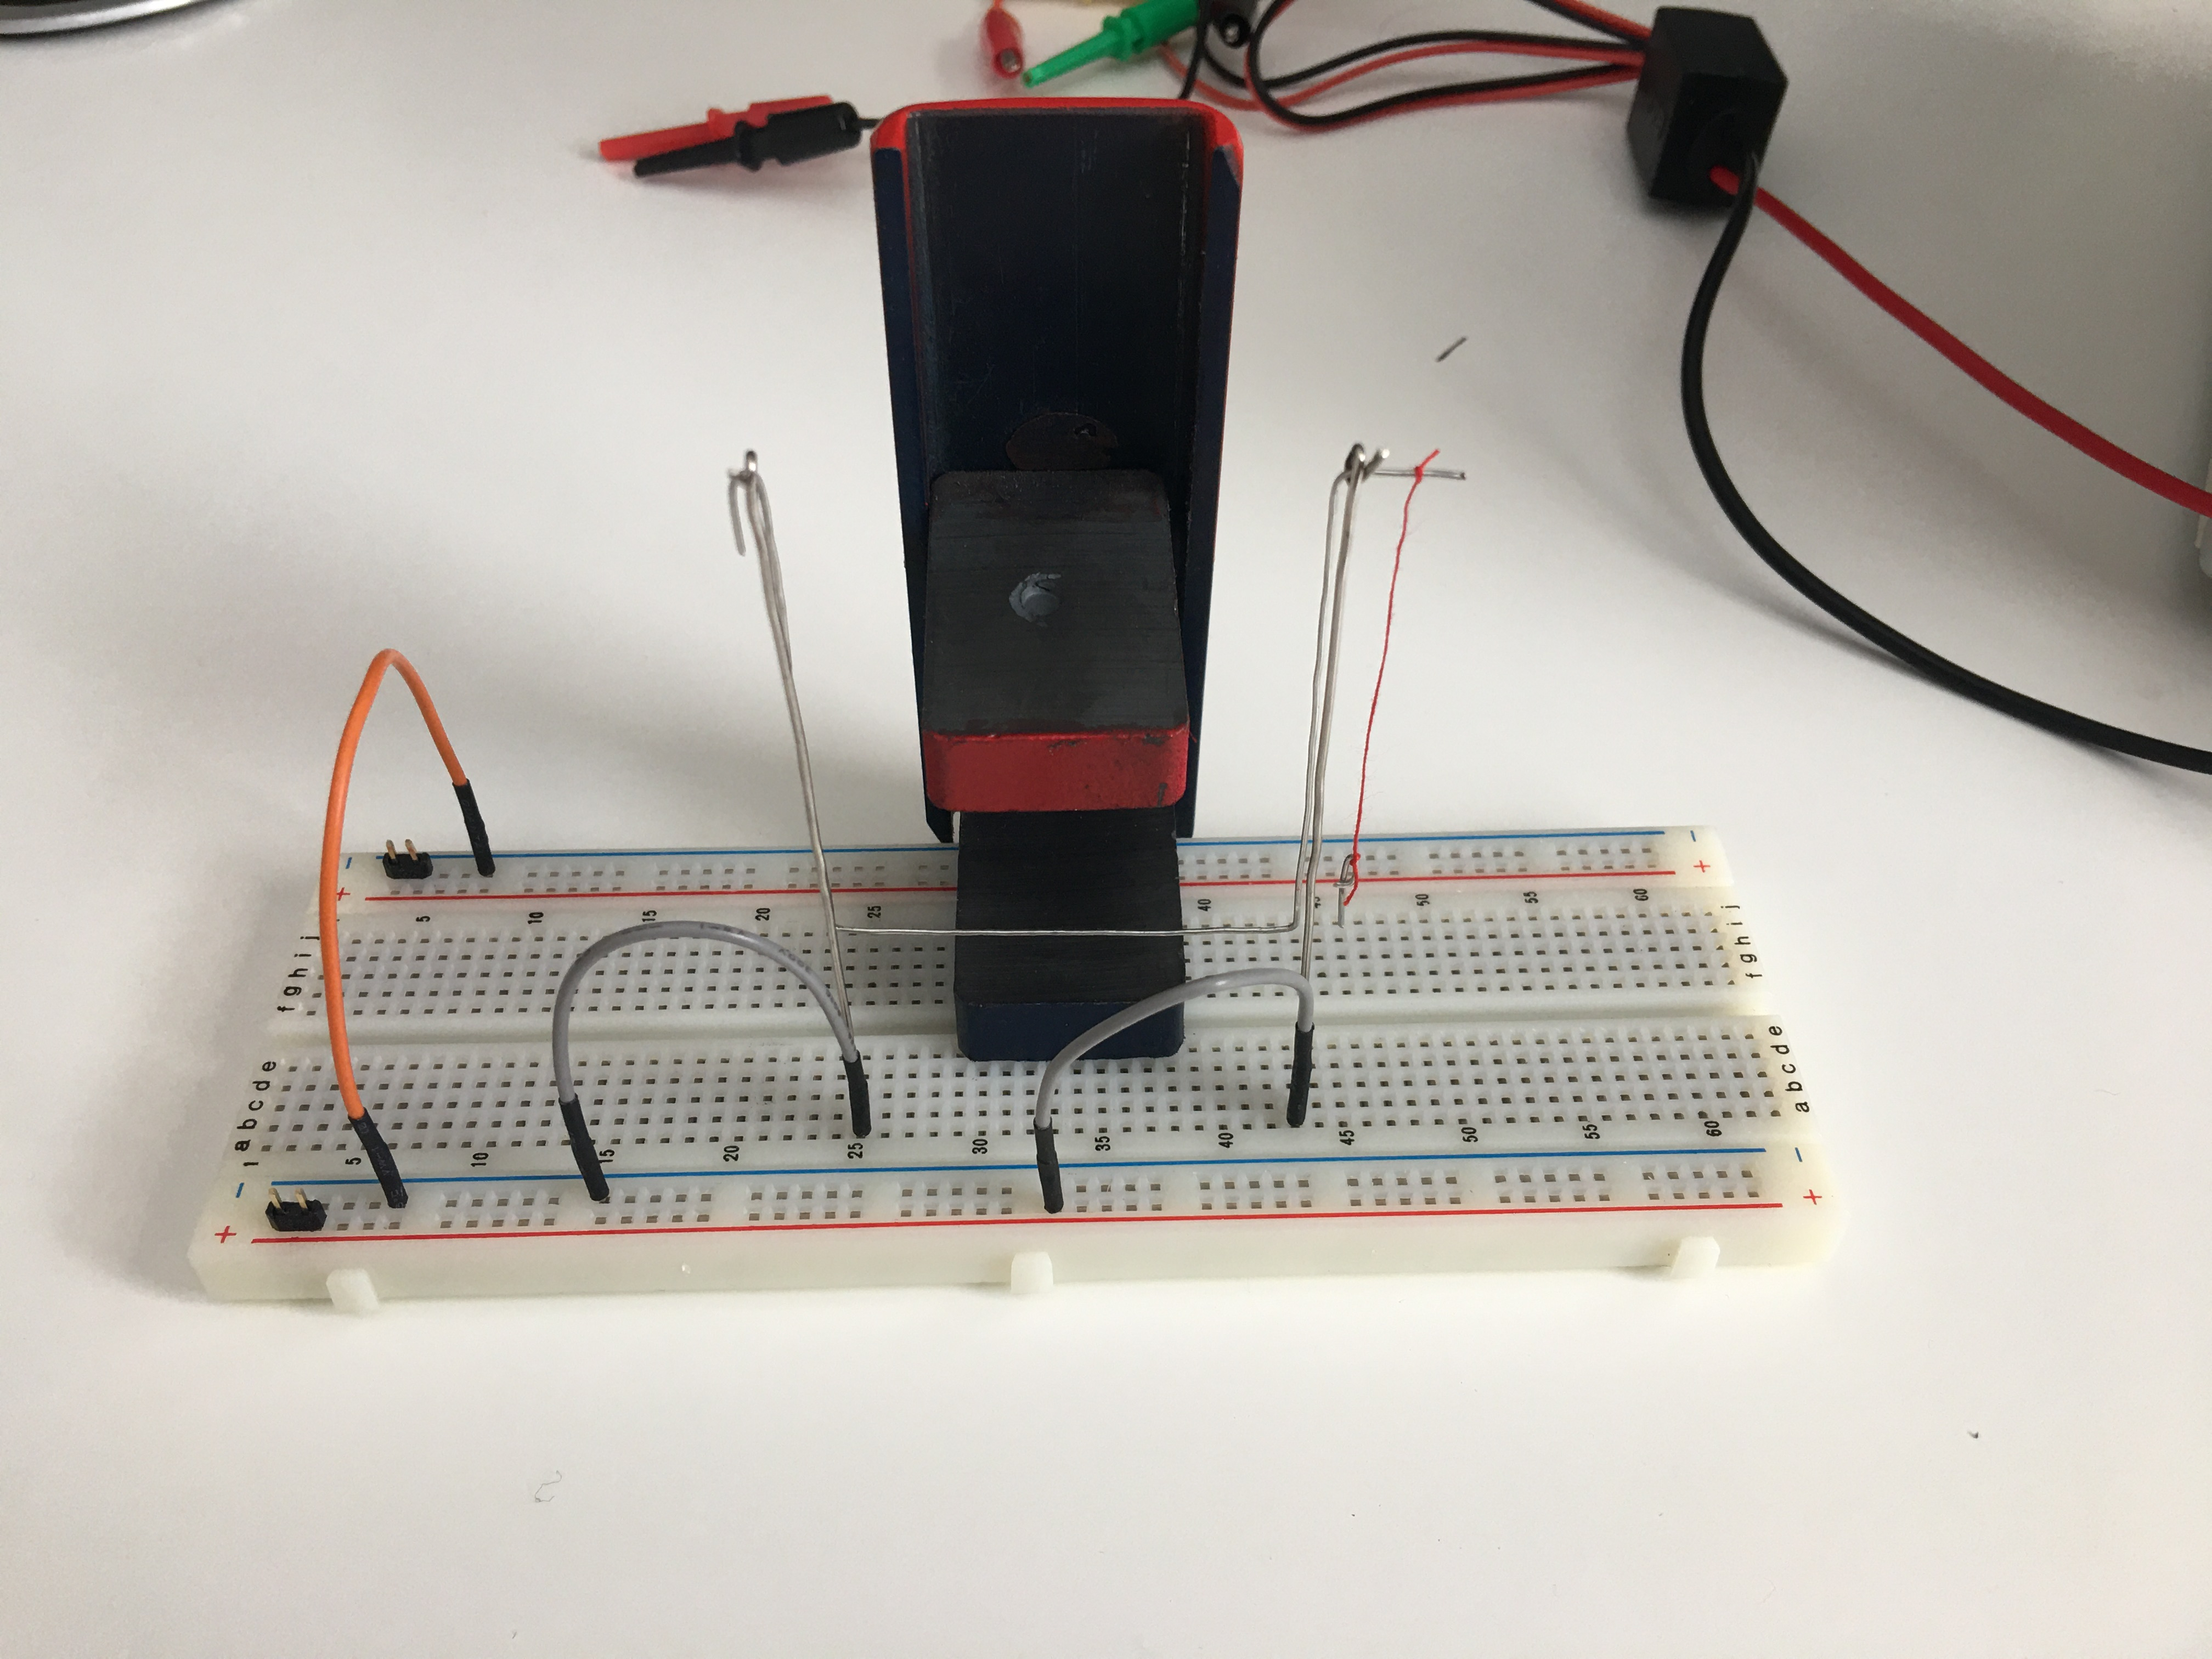
\includegraphics[width=0.5\textwidth]{figures/IMG_5514.JPG}
		\caption{Image of the apparatus. The positive side of the wire is indicated by the red thread.}
		\label{fig:apparatus}
	\end{figure}
	\item Gather two large flat surface area magnets whose poles are on the largest face and a metal bracket which the magnets will be mounted onto.
	The magnets must have a large enough surface area to account for the expected deflection angle range.
	\begin{enumerate}
		\item Take note of the poles of each magnet.
		Identify which face of each magnet is north and south.
		\item Mount one magnet onto the bottom of the metal bracket with its south pole facing up.
		Mount the other magnet so that its south pole is also facing up, with the minimum amount of distance between the two magnets so that a uniform magnetic field is created, but does not result in the two magnets breaking off the mount and attracting each other.
		Also ensure that the distance between the two magnets is enough to account for the movement of the wire as its deflection angle increases.
		\item Place the mount onto the breadboard and in front of the wire.
		The wire should be within but on the edge of the magnetic field between the two magnets.
	\end{enumerate}
	\item Gather the power supply and necessary cables to provide current to the apparatus.
	\begin{enumerate}
		\item Use jumper wires to connect the lanes of the supports to the power rails on the breadboard.
		When viewing the apparatus perpendicular to the wire, make sure the pendulum is connect to the power rails so that conventional current flows from right to left.
		\item Verify that there are no potential short circuits on the breadboard.
		\item Connect the power supply to the power rails and provide $0.5\si{\volt}$ to the breadboard to test the setup.
		If everything is set up correctly, the wire should have deflected from the normal and away from the supports, into the magnets.
		If the wire deflects into the supports, switch around the direction of current in the pendulum setup.
		If the wire does not move, either the circuit is open somewhere, the knuckles or hooks are too small, the wire is not making contact with the supports due to insulation, or the paperclips are not conductive.
		Troubleshoot each potential issue.
	\end{enumerate}
	\item Prop a camera or imaging sensor at least $15\si{\centi\meter}$ away from the apparatus and facing parallel to the length of the wire.
	Make sure the position and orientation of the camera to the apparatus remains the same throughout the experiment.
	The vertical segment of the wire should be on a single perpendicular plane relative to the camera and at the center of the image.
	\item Use the camera to photograph the deflection angle of the wire while at rest. \label{step:measure0}
	\item Provide enough voltage to the breadboard such that there is about $0.20\si{\ampere}$ going through the wire.
	Because the current may fluctuate as the wire swings, it is fine to around be within $\pm0.10\si{\ampere}$, so long as the current is no longer fluctuating and the wire is in a static equilibrium. \label{step:measure}
	\vspace{-1em} % something wrong went on here
	\begin{enumerate}
		\item If the power supply does not measure current, use a digital multimeter and connect one end to a support and the other to its respective power rail.
		\item Use the camera to photograph the deflection angle of the wire. 
	\end{enumerate}
	\item Repeat step \ref{step:measure} with $0.40\si{\ampere}$, $0.60\si{\ampere}$, $0.80\si{\ampere}$, $1.00\si{\ampere}$, $1.20\si{\ampere}$, and $1.40\si{\ampere}$.\label{step:repeat}
	\item Repeat steps \ref{step:measure0}, \ref{step:measure}, and \ref{step:repeat} four more times, ending with five trials.
\end{enumerate}

\subsection*{Safety Considerations}

As mentioned before, the current should be kept below $2.00\si{\ampere}$ to reduce the chance of a burn.
Parts of the apparatus may become hot, mainly the point of connection between the wire and the supports, so avoid touching those areas.
Keep the overall power output of the power supply below $4.00\si{\watt}$ so that there is not enough power to induce current through your body.
When handling strong magnets, avoid placing any bodily extremities between them, as they can potentially cause injury.
